\documentclass{article}
\usepackage{amsmath, amssymb}
\usepackage{tcolorbox}
\usepackage{tikz}
\usepackage{geometry}
\usepackage{xcolor}
\usepackage{titlesec}
\usepackage{enumitem}
\usepackage{colortbl}
\usepackage{fancyhdr}
\usepackage{sectsty}
\usepackage{lmodern} % Modern font
\usepackage{microtype} % Improves text appearance
\usepackage{graphicx} % For including images

% Page Geometry
\geometry{a4paper, margin=1in}

% Color Definitions
\definecolor{sectioncolor}{RGB}{60,60,60}
\definecolor{definitioncolor}{RGB}{255,102,0}
\definecolor{tableheadercolor}{RGB}{230,230,230}

% Section Formatting
\sectionfont{\color{sectioncolor}\normalfont\Large\bfseries}
\subsectionfont{\color{sectioncolor}\normalfont\large\bfseries}

% Highlighted Box for Definitions
\newtcolorbox{definitionbox}[1][]{
    colframe=definitioncolor!80,
    colback=definitioncolor!10,
    fonttitle=\bfseries,
    title=#1
}

% Header and Footer
\pagestyle{fancy}
\fancyhf{}
\fancyhead[L]{IB Analysis and Approaches HL2}
\fancyhead[R]{Inverse Trigonometric Functions}
\fancyfoot[C]{\thepage}

% Title
\title{\textbf{IB Analysis and Approaches HL2 \\ Inverse Trigonometric Functions}}
\author{}
\date{}

\begin{document}
\maketitle

% Introduction Section
\section*{Definition \& Purpose}

% add space for students to write
\begin{tcolorbox}[colback=white, colframe=sectioncolor!50, width=\textwidth, height=2in, valign=center, halign=left]
\end{tcolorbox}

% Understanding Trigonometry Section
\section*{Triangle}
Suppose we have a right triangle with an angle $\theta$ and sides of length $a$, $b$, and $c$ as shown below.

\begin{center}
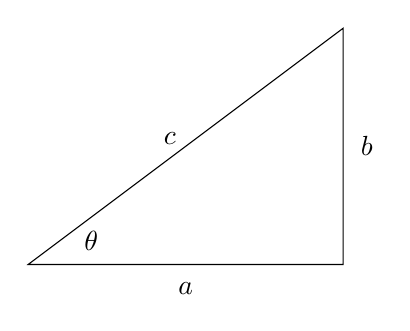
\begin{tikzpicture}
\draw (0,0) -- (4,0) -- (4,3) -- cycle;
\node at (2,-0.3) {$a$};
\node at (4.3,1.5) {$b$};
\node at (1.8,1.6) {$c$};
\node at (0.8,0.3) {$\theta$};
\end{tikzpicture}
\end{center}

In regular trigonometry:
\begin{align*}
\sin(\theta) &= \frac{b}{c}, \\
\cos(\theta) &= \frac{a}{c}, \\
\tan(\theta) &= \frac{b}{a}.
\end{align*}

\begin{center}
\begin{tabular}{|p{0.35\textwidth}|p{0.25\textwidth}|p{0.25\textwidth}|}
\hline
\rowcolor{tableheadercolor}
\textbf{Trigonometric Function} & \textbf{Domain} & \textbf{Range} \\
\hline
$\arcsin(x)$ & & \\
\hline
$\arccos(x)$ & & \\
\hline
$\arctan(x)$ & & \\
\hline
\end{tabular}
\end{center}

\subsection*{Domain and Range Visualization}

\begin{center}
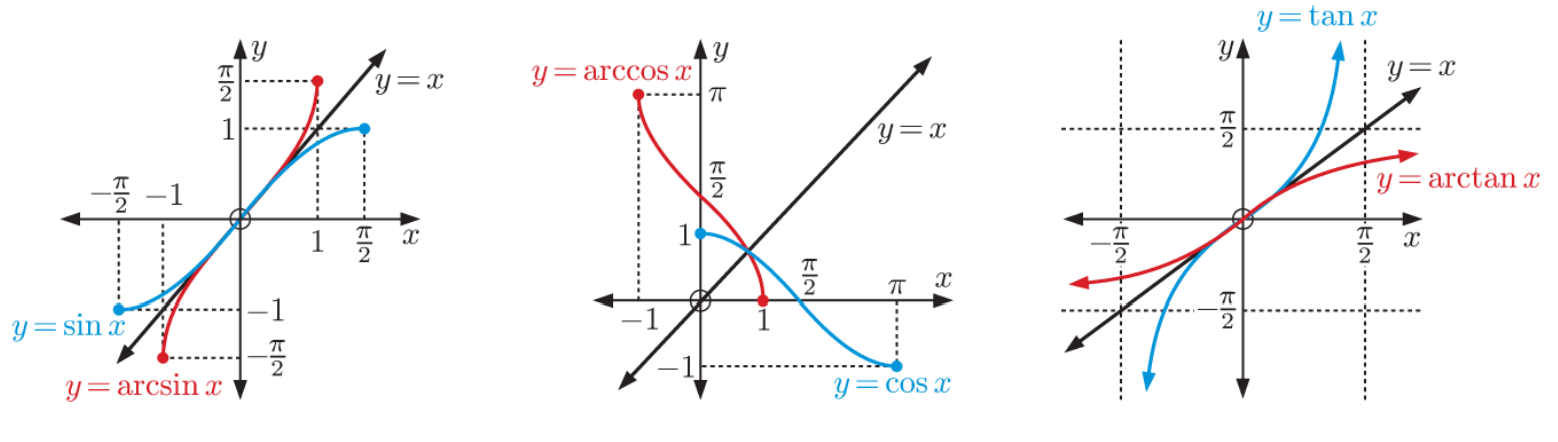
\includegraphics[width=\textwidth]{Screenshot 2024-05-14 192525.png}
\end{center}

\section*{Example Problems}

\begin{enumerate}
    \item \textbf{Satellite Communication}: A satellite orbits the Earth, and the angle between the line from the satellite to a ground station and the line from the satellite to the Earth's center is \(\arcsin\left(\frac{2}{3}\right)\). If the distance from the satellite to the Earth's center is 10,000 km, what is the distance from the satellite to the ground station?
    
    \begin{tcolorbox}[colback=white, colframe=sectioncolor!50, width=\textwidth, height=2in, valign=center, halign=left]
    \end{tcolorbox}

\end{enumerate}

\section*{Key Takeaways}
\begin{definitionbox}[Inverse Trigonometric Functions]
\begin{itemize}
    \item $\arcsin(x)$: Inverse of $\sin(x)$. Domain: $-1 \leq x \leq 1$, Range: $-\frac{\pi}{2} \leq y \leq \frac{\pi}{2}$.
    \item $\arccos(x)$: Inverse of $\cos(x)$. Domain: $-1 \leq x \leq 1$, Range: $0 \leq y \leq \pi$.
    \item $\arctan(x)$: Inverse of $\tan(x)$. Domain: $-\infty < x < \infty$, Range: $-\frac{\pi}{2} < y < \frac{\pi}{2}$.
\end{itemize}
\end{definitionbox}

\end{document}
